\documentclass[a4paper,answers]{exam}
\usepackage{hyperref}
%\usepackage{eulervm}
\usepackage{mathpartir}
%\usepackage{pgffor}
%\usepackage{ascii}
\usepackage{xcolor}
\usepackage{placeins} %for FloatBarrier
\usepackage{version,a4wide}
%,pifont}
%\usepackage{textcomp}
\usepackage{amsmath,amsthm}
\usepackage{stmaryrd}
\usepackage{amssymb}
\usepackage{lipsum}
\renewcommand{\ttdefault}{cmtt}
\pointname{ marks}
\qformat{\textbf{Question \thequestion} $\ $ (\thepoints)\hfill}
\newcommand\llangle{\langle\!\langle}

\usepackage{tikz}
\usetikzlibrary{automata,positioning,shapes.geometric,fit,calc}

\tikzset{initial text={},on grid, auto, thin,
    every state/.style={circle,minimum size=.6cm,
      %draw=blue!50,
      draw=black,
      thin,fill=none,text=black},
    node distance=1.2cm,on grid,auto,
    bend angle=35}
\newcommand\rrangle{\rangle\!\rangle}
\newcommand{\mapstos}[0]{\stackrel{\star}{\mapsto}}
\newcommand{\mapstoc}[0]{\stackrel{!}{\mapsto}}

\begin{document}
\begin{flushright}
   $\ $\\[5em] Name: Jinghan Wang \\[1em]
    Student Number: z5286124 \\[1em]
    Signature: 
\includegraphics[width=0.15\textwidth]{sign}\\[3em]
\end{flushright}
\begin{center}
\textsc{\Large The University of New South Wales}\\[3em]
{\Huge COMP3151/9154\\[0.3em] Foundations of Concurrency}\\[3em]
{\Large \textbf{Final Exam}}\\[1em]
{\large \textit{Term 2, 2022}}\\[5.7em]
{\large
\begin{description}
    \item[Time Allowed:] 24 Hours. Submit by 8AM Sydney time on August 23.
    \item[Total Marks Available:] 100
    \item[] $\!\!\!\!\!$ Brief answers are \textbf{strongly} preferred. Extreme verbosity may cost marks.
    \item[] $\!\!\!\!\!$ Produce a typeset PDF file, via \LaTeX{} or otherwise, with your answers.
    \item[] $\!\!\!\!\!$ Submit with \texttt{give cs3151 exam exam.pdf} or with the \texttt{give} web interface.
    \item[] $\!\!\!\!\!$ The exam is open-book. You may read anything you like, and in general use any passive resource.
    \item[] $\!\!\!\!\!$ You \textbf{may not} use active resources---don't solicit, offer, or accept help of any kind, with one exception: you may ask private questions on Ed. Johannes will monitor Ed regularly, except when he sleeps (around 10PM--6AM).
    \item[] $\!\!\!\!\!$ Include the following statement in your PDF file:\\
\emph{I declare that all of the work submitted for this exam is my own work, completed without assistance from anyone else.}
   \item[] $\!\!\!\!\!$ You must adhere to the UNSW student conduct requirements listed at\\ \url{https://student.unsw.edu.au/conduct}.
\end{description}
}
\end{center}
\newpage

%\setcounter{latest@ques}{1}

\begin{questions}

\section*{Part I}

\question[10]
Answer the following, briefly and in your own words.

\begin{parts}

\part[2] What is a linear-time property?
\begin{solution}
    The linear-time Properties used to describe requirements of a model of a computer system and specifies the permissible or expected behavior of the system under consideration which mainly include safety properties and liveness properties.
\end{solution}

\part[2] Why does Owicki-Gries require interference freedom checks?
\begin{solution}
    When we need to understand the correctness of a concurrent algorithm, it is difficult to infer multiple interleaved processes and easily make mistakes. Interference freedom check is mainly used to prove the correctness of one process exclusion without interfering by others process.
\end{solution}

\part[2] How do distributed consensus algorithms get around the FLP theorem?
\begin{solution}
    Some distributed consensus algorithms use random algorithms to make all nodes agree on the probability that a certain output value is correct. The algorithm sets a threshold for the number of members that must reach consensus.
\end{solution}

\part[2] What limitation of Spin will we run into if we try to model check the Bakery algorithm?
\begin{solution}
    Always exists process in the critical section, other process which is applying to enter the critical section will change itself to the maximum number of the array plus 1, as the process is quickly, this number is unbounded size. 
\end{solution}

\part[2] What is the difference between a permission-based and a token-based distributed mutual exclusion algorithm?
\begin{solution}
    For token-based Distributed Mutual exclusion algorithm, only processes with tokens can enter the Critical section. Processes only need to send requests and waiting for the token to be accepted. They are free of deadlocks due to the presence of unique tokens in distributed systems. Processes that request access to CS can be ordered and prioritized.\\\\
    For permission-based Distributed Mutual exclusion algorithm, responses from all processes are required to enter the critical section, and priority can be determined. Access to Critical sections is determined by sending information between programs.
    
\end{solution}
\end{parts}

\clearpage
\question[15]

These questions are about the critical section algorithm in Table 1.
The purpose of this algorithm is to get away with the least amount of shared state
possible, which turns out to be one bit per process.

\begin{table}
\begin{center}
\begin{tabular}{| c l |  c l |}
\hline 
\multicolumn{4}{| c |}{ $\textbf{bool}\ \mathit{x,y} := \mathsf{false}$}\\
\hline
\multicolumn{2}{| l |}{\textbf{forever}\ \textbf{do}} & \multicolumn{2}{| l |}{\textbf{forever}\ \textbf{do}} \\ 
p$_1$ & \textit{non-critical section} & q$_1$ & \textit{non-critical section} \\ 
p$_2$ & $x := \mathsf{true}$ & q$_2$ & $y := \mathsf{true}$ \\
p$_3$ & \textbf{await} $\neg y$ & q$_3$ & \textbf{if} $x$ \textbf{then} \\
p$_4$ & \textbf{\emph{critical section}} & q$_4$ & \quad $y := \mathsf{false}$ \\
p$_5$ & $\mathit{x} := \mathsf{false}$ & q$_5$ & \quad \textbf{await} $\neg x$ \\
 &  & q$_6$ & \quad \textbf{goto} q$_2$ \\
 &  & q$_7$ & \textbf{\emph{critical section}} \\
 &  & q$_8$ & $y := \mathsf{false}$ \\\hline
\end{tabular}
\end{center}
\caption{A critical section algorithm.\label{onebit}}
\end{table}

\begin{parts}
    \part[5] Of the four main critical section desiderata
    (mutual exclusion, deadlock freedom, eventual entry, and absence of unnecessary delay),
    which ones are satisfied by this algorithm?
    For any properties that are not satisfied, describe a behaviour that is in violation.

    \begin{solution}
        Mutual exclusion: the algorithm is mutual exclusion. It exists four situation, when $x,y = false$, no one can enter to the critical section. When $x = true$, $x$ can enter into critical section because although $y = true$, $y$ will change it self to false and allow $p$ can enter into. when $x = false, y = true$, $y$ can goto critical section, during this section, $y=true$, $p$ stop at $p_3$ and cannot enter.\\\\
        Deadlock freedom, the algorithm is deadlock freedom. Suppose the process have deadlock, when both $x$ and $y$ equal false, $q_2$ and $p_2$ can change themselves to $true$ it is not satisfied by the deadlock; When $x$ and $y$ is true, $q$ checks that $x=true$, it will change $y$ to false. It also did not satisfy. When $x$ and $y$ is different, the $p$ and $q$ can enter into critical section, it also did not satisfy the definition of deadlock. Therefore, it is deadlock freedom.\\\\
        Eventual entry: This algorithm does not satisfy eventually entry. When $p$ comes out of the critical section and changes $x = false$, $q$ detects $x = false$, changes itself to $y = true$ again, and detects the state of $x$. if $x$ changes to true during this time, $q$ will continue to wait. There is a possibility that this state will continue all the time, resulting in the failure of $q$ to finally enter.\\\\
        Absence of unnecessary delay: It is satisfied. When $p$ or $q$ in non-critical section, the $x$ or $y$ is false. When the $x$ or $y$ want to enter into critical section and the other one is in non-critical section, $\lnot y = true$ or $(x = ture) = false$, it can enter into critical section.
    \end{solution}

    \clearpage
    \part[5]
    Suppose we rewrite process $p$ to be exactly like process $q$, but with the roles
    of $x$ and $y$ swapped. Would this change your answer to the previous question?
    \begin{solution}
        In this case, mutual exclusion is satisfied because must satisfy one is true and other is false can go into the critical section.\\
        It does not satisfy deadlock freedom, because suppose the $p$ and $q$ change themselves to true together. If both detects that the other side is true, they change it to false, and then both detects that the other side is false, they change it to true. This is an infinite loop and does not meet the circular waiting principle of deadlock freedom.\\
        This algorithm also does not satisfy eventually entry. Because it also exists the possibility that one process gives way to another at all time.\\
        Absence of unnecessary delay: it is satisfied and same as above.

    \end{solution}

    \part[5] Why are there no algorithms with only a single bit of shared state?
    You don't have to produce a formal proof, but try to make a convincing
    informal argument.
    
    For the purposes of this question, we consider an algorithm correct
    if it satisfies at least mutual exclusion and deadlock freedom (in
    the sense ``if a process is trying to enter the critical section,
    then assuming weak fairness, some process will eventually enter the critical section'').
    \begin{solution}
        In my opinion, according to the title, we can assume that the shared value is read / write only with atomic. If we want to meet the requirements of the topic, in the first case, the shared value is Boolean. In this case, we cannot know the status of each process. In the second case, the shared value is the serial number or unique character of different processes, and additional characters that allow the program to apply for entry into the critical section need to be set. The program needs to check whether it can apply, and then write its own serial number to prevent others from entering. In this case, in addition to entering the critical section.
    \end{solution}
\end{parts}

\clearpage
\question[15]

Assume you have an underlying monitor implementation $I$ with priority ordering $E
= W < S$.
Suppose we would like a monitor $M$ to behave as if it had priority ordering 
$E < W < S$.
Show how to implement our desired monitor $M$ using our underlying implementation $I$.


Present your solution in the form of pseudocode snippets to be executed upon
monitor entry, monitor exit, signalling and waiting. That is, assume
that whenever monitor $M$ would like to execute, e.g., $\mathbf{waitC}(\mathit{cond})$, it
runs your code snippet instead.
You may introduce auxiliary variables and condition variables as
needed.
Some of the snippets might be empty, in which case they can be left out.
\begin{solution}
    \newline According to the topic, $I.append$ is inserting data to monitor $I$, $I.take$ is getting the data from monitor $I$; \\
    When monitor $M$ run, append\_i will be direct execution. Process with dataType use $M.append$ enter into monitor $M$ and $M.take$ can accept to enter into critical section.\\
    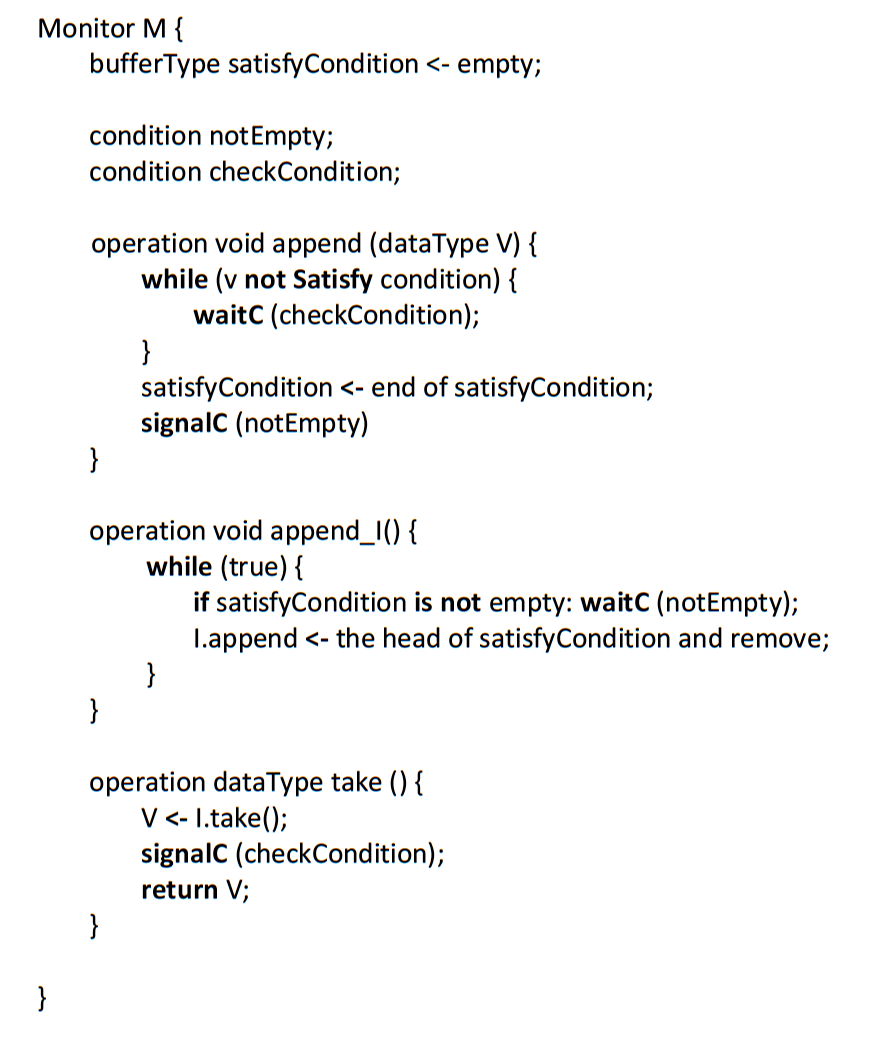
\includegraphics[width=0.9\textwidth]{DV_command1}
\end{solution}

\clearpage
\question[10]

\begin{parts}
\part[5] Consider the LTL formula $\Diamond\Box\Diamond\varphi$.
  Give a simpler but logically equivalent formula. Explain why it's equivalent.
\begin{solution}
    $\lnot \varphi\ \mathcal{U}\ \Box(\varphi \wedge \lnot \varphi)$\\
    $\Diamond\Box\Diamond\varphi$ means exists a time in the future, always eventually $\varphi$. Now, it satisfied $\lnot \varphi$ and in the future it will keep repeating states $\varphi$ or $\lnot \varphi$ forever。
\end{solution}
\part[5] Let the CCS process $P$ be defined as follows:
\[P = (x.P){\backslash}x\]

Simplify the following CCS expression step by step:
\[(x.(P{\backslash}x)){\backslash}x\]

\emph{Hint:} it simplifies a lot!
A selection of algebraic laws about restriction that you may use can be found in Table 2.

\begin{solution}
    According to the topic,
\begin{center}
    $P = (x.P){\backslash}x$
    \end{center}
    As $x \in \{x,\overline{x}\}$, it means both $x$ and $P$ except that the actions $x$ and $\overline{x}$ may not be executed,
    \begin{center}
        $P = (x){\backslash}x.(P){\backslash}x$\vspace{1em}
    \end{center}
    According to the Table 2 $P{\backslash}x{\backslash}x = P{\backslash}x$. therefore, $P{\backslash}x = P{\backslash}x{\backslash}x$, \vspace{1em}
    \begin{center}
        $P = x{\backslash}x.(P{\backslash}x{\backslash}x)$\vspace{1em}\\
        $P = x{\backslash}x.(P{\backslash}x){\backslash}x$\vspace{1em}\\
    \end{center}
    Both $x$ and $(P{\backslash}x)$ need except that actions $x$ and $\overline{x}$, it can merge,\vspace{1em}
    \begin{center}
        $P = (x.(P{\backslash}x)){\backslash}x$
    \end{center}
\end{solution}

\begin{table}
\begin{center}
\begin{mathpar}
  (a.P){\backslash}x = a.(P{\backslash}x) \quad\mbox{if $x \notin \{a,\overline{a}\}$}
  \and
  P{\backslash}x{\backslash}x = P{\backslash}x
  \and
  P{\backslash}x{\backslash}y = P{\backslash}y{\backslash}x
\end{mathpar}
\end{center}
\caption{A critical section algorithm.\label{2}}
\end{table}

\end{parts}

\clearpage
\FloatBarrier
\section*{Part II}

These questions are about the paper \emph{Simple, Fast, and Practical Non-Blocking and Blocking Concurrent Queue Algorithms} by Maged M. Michael and Michael L. Scott (PODC 1996: 267-275).

\question[15]

\begin{parts}
\part[5] Section 1 of the paper includes an extensive summary of the state of the art
in 1996. How did Michael and Scott's paper improve the state of the art?  
\begin{solution}
    The improvement of Michael and Scott's paper is two new concurrent FIFO queue algorithms, one is non-blocking and the other uses a pair of locks. Although the new two-lock algorithm cannot compete with the non-blocking alternatives on a multi programmed system, outperforms a single lock when several processes compete for access simultaneously. 
\end{solution}

\part[3] What is the difference between a block-free algorithm and a wait-free algorithm?
Of the two, which kind of algorithm did the specification of Assignment 1 ask for?
\begin{solution}
    Block-free algorithm is means that the failure or suspension of any process will not cause failure or suspension of another thread. \\
    Wait-free algorithm is is the strongest Block-free guarantee of progress, except satisfy the requests of Block-free algorithm, every thread is also guaranteed to make progress over an arbitrary period of time, regardless of the timing or ordering of thread execution.\ \ In my opinion, Assignment 1 is Block-free algorithm.
\end{solution}

\part[2] Based on the performance analysis in Section 4, are there any situations where
Michael and Scott's non-blocking algorithm is \emph{not} preferrable?
\begin{solution}
    As can be seen from the three figures, when it is two processes, single-lock is slightly better than two-lock algorithm, but it is also in the second position. For multiple processes, the two-lock algorithm has great advantages and its performance is excellent enough. It appears to be a reasonable choice for machines that are not multi programmed, and that lack a universal atomic primitive.
\end{solution}


\part[5]
The compare-and-swap (CAS) on line E17 of the non-blocking algorithm has the accompanying comment
``Try to swing Tail to the inserted node''.
This suggests that, if the CAS fails, an enqueue operation can terminate even
if its work is unfinished.
Is this a problem? Explain why or why not.
\begin{solution}
    First, according to the restrictions of initialize and D6, D7 in dequeue, the queue will not be empty, and  Q$\rightarrow$tail must point to a node. When the program is in E7, it checks whether the tail points to the last node. If not, it points Q$\rightarrow$tail to the next node. If yes, the address of the new node is written into the next of the last node in queue. Only this way can break the loop. Because of the existence of the lock, there is no problem that when this process writes to the tail, another process writes at the same time to cause an error. When the loop ends, Q$\rightarrow$tail must point to the penultimate node. Even if an error occurs in E17 and Q$\rightarrow$tail fails to be recorded as a new tail. But in fact, the only the new node next.ptr is NULL and it is the tail of queue. The loop will keep when the other process want to insert node, must insert after the node next.ptr is NULL.
\end{solution}

\end{parts}

\clearpage
\question[25]

The ABA problem is discussed a lot in the paper.

\begin{parts}
\part[4]
What is the ABA problem? Explain informally and in your own words.
\begin{solution}
    Suppose there are two threads $x$, $y$, and a shared memory. The initial shared memory is 0, and thread x reads the value 0 and prepare to write. May be due to some blocks, during this period, $y$ writes 1 to the shared memory and then write 0 to the shared memory. When $x$ is read again, it is still 0 and thread x continues to write. Although $x$ works normally, the shared memory is actually modified, which may lead to incorrect behavior.
\end{solution}

\part[3]
How does the authors' use of modification counters help mitigate the ABA problem?
\begin{solution}
    Every time CAS is performed, the program will $node.count + 1$, even in the case of ABA, when $a$ checks again, the count will change, and the process will know that there are modifications during this period.
\end{solution}

\part[5]
Ominously, the safety analysis in Section 3.1 is predicated upon the
assumption that the ABA problem will never occur.  Describe a scenario
where, in the lock-free algorithm, the queue can end up corrupted if
the ABA problem occurs.

\emph{Hint:} make the modification counters wrap around.
\begin{solution}
    When the program is unlocked, it is assumed that program $a$ ends E9 and meets the compare conditions to want to swap and is blocked by some reasons. Program $b$ executes the insertion normally. At this time, process $a$ still thinks that the next is NULL and writes its new node address into the next. No other node's next records the node that program $b$ normally inserts. This node's value will never be obtained by dequeue.
\end{solution}

\begin{table}
\begin{center}
  \begin{tabular}{| c l |  c l |}
  \hline 
  \multicolumn{4}{| c |}{ $\textbf{int}\ \mathit{n} := 0$} \\
  \hline
  \multicolumn{2}{| c |}{ $\textbf{int}\ \mathit{i} := 10$} & \multicolumn{2}{| c |}{ $\textbf{int}\ \mathit{j} := 10$}\\
  \hline
  \multicolumn{2}{| l |}{\textbf{while}\ $i \neq 0$} & \multicolumn{2}{| l |}{\textbf{while}\ $j \neq 0$} \\ 
  p$_1$ & \textbf{repeat} & q$_1$ & \textbf{repeat} \\ 
  p$_2$ & \quad $x := n$ & q$_2$ & \quad $y := n$ \\
  p$_3$ & \textbf{until}\ $\mathsf{CAS}(n,x,(x + 1) \mathop{\mathsf{mod}} 3)$ & q$_3$ & \textbf{until}\ $\mathsf{CAS}(n,y,(y + 1) \mathop{\mathsf{mod}} 3)$ \\
  p$_4$ & $i := i - 1$ & q$_4$ & $j:=j-1$ \\ \hline
  \end{tabular}
\end{center}
\caption{A critical section algorithm.\label{3}}
\end{table}

\part[3]
Sometimes, ABA-type situations are innocuous. Consider the program in
Table 3.  Describe how the $\mathsf{CAS}$ at $p_3$ may succeed,
despite $n$ having changed since the read on line $p_2$.
\begin{solution}
    Because the program is finite, the program will eventually end, it's just a priority matter of $p$ and $q$. Suppose between $p_2$ and $p_3$, $q$ does this multiple times and changes the $n$ value to the same value. The program will not cause deadlock, $q$ will end faster, and $p$ will not be affected.
\end{solution}

\part[10]
The end result of running the program in Table 3
is unaffected by whether ABA situations happen or not. Or to be
precise, the program will satisfy the following Hoare triple:
\[
\{n = 0\}\;P || Q\;\{n = 2\}
\]
Where $P$ and $Q$ are the left and right processes, respectively.
Formulate a single global invariant that suffices to establish
this Hoare triple.
\begin{solution}
    $\{True\}\;P || Q\;\{x=1\ \| \ y=1\}$
\end{solution}
\end{parts}

\question[10]

The last item in Section 3.1 states ``\emph{Tail} always points to a
node in the linked list, because it never lags behind \emph{Head}, so
it can never point to a deleted node''.

\begin{parts}
\part[5]
This statement is false for
the two-lock concurrent queue.  Describe how a state can be reached
where \emph{Tail} points to a deleted node.

\emph{Hint:} look for a state where one of the locks is held.
\begin{solution}
    When the D6 inspection is completed, $head.ptr = tail.ptr$, E9 inserts a new node into tail$\rightarrow$next.ptr, and then D7 detects head$\rightarrow$next.ptr is not equal to NULL and remove head.ptr. At this time, E17 operation has not been performed. \emph{Tail} still points to original node but the node had been removed.
\end{solution}

\part[5] Is it possible to reach a state where \emph{Head} points to a deleted node?
Explain why or why not.
\begin{solution}
    No, because the program changes the \emph{Head} to next.ptr first and is followed by the free operation. When the node is removed, the \emph{Head} must already point to the next node. Therefore, there is no case where the \emph{Head} points to the deleted node
\end{solution}
\end{parts}

\end{questions}

\textbf{Dont forget to submit your work and include the statement given on the front page}.\\

\centerline{\bf \large --- END OF EXAM ---}

\end{document}

